\documentclass[10pt]{exam}
\usepackage[phy]{template-for-exam}
\usepackage{graphicx}

\title{Reading Guide for Newton's Laws}
\author{Rohrbach}
\date{\today}

\begin{document}
\maketitle

\vspace{-2em}

\begin{questions}
  
\uplevel{
  \section*{Newton's First Law}
  
  Read p. 26 in \emph{Conceptual Physics} then answer the following questions:
  
}

\question
  What is the key word in the Law of Inertia?
  \vs

\question
  The figure below shows someone pulling a tablecloth out from under a place setting.  Use the key word for the Law of Inertia to explain how this works.

  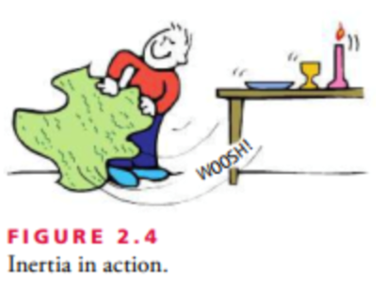
\includegraphics[width=4.5cm]{images/2-4.png}
  \vs
  
\question
  Pick one of these figures and explain what is happening using Newton's First Law.

  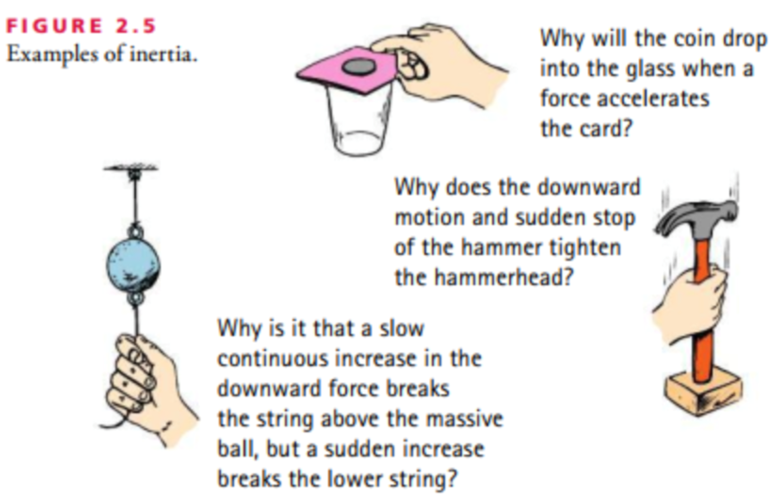
\includegraphics[width=7cm]{images/2-5.png}
  \vs

\uplevel{
\section*{Newton's Second Law}

Read pp. 63-64 in \emph{Conceptual Physics} then answer the following questions:
  
}

\question
  What does ``directly proportional'' mean?
  \vs

\question
  What does ``inversely proportional'' mean?
  \vs

\question
  How is acceleration related to net force and mass?
  \vs

\question
  What is this figure trying to show?

  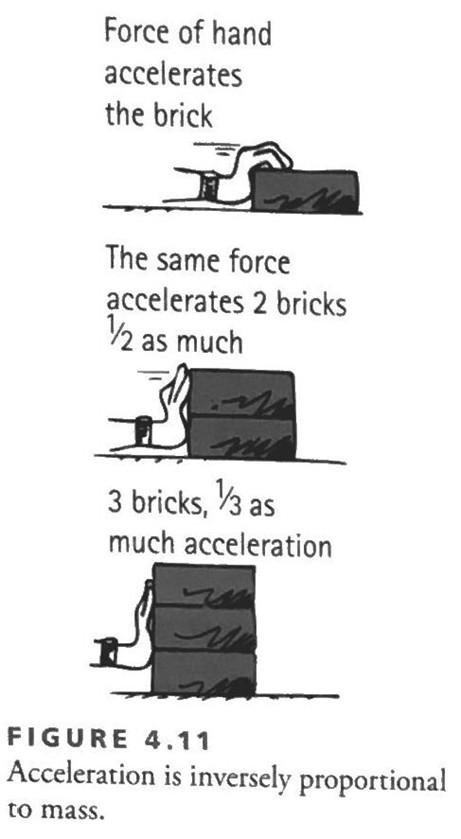
\includegraphics{images/4-11.png}
 
\uplevel{
  \section*{Newton's Third Law}

  Read pp. 75-76 in \emph{Conceptual Physics} then answer the following questions:
  
}
 
\question
  What is an \emph{interaction}?
  \vs

\question
  Use the concept of interaction to explain why this guy doesn't topple over.

  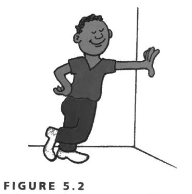
\includegraphics[width=3cm]{images/5-2.png}
  \vs
 
\question
  When you walk, you do so by exerting an action force with your feet pushing against the floor backwards.  What is the reaction force?
  \vs

\question
  If a car's tires push on the road as an action force, what is the reaction force?
  \vs


\end{questions}

\end{document}